\subsubsection{振動子}\label{vibrator}
\begin{table}[H]
  {\renewcommand\arraystretch{1.4}
    \begin{tabular}{|p{\colF}|p{\colG}|}	\hline
    名称 & 振動子(しんどうし)\\ \hline
    接続箇所 & デジタルコネクタ (3pin)\\ \hline
    機能概要 & 振動モーターでふるえる\\ \hline
    \end{tabular}
  }
\end{table}

\begin{table}[H]
  {\renewcommand\arraystretch{1.4}
    \begin{tabular}{|p{\colF}|p{\colG}|}	\hline
    サンプルコードの場所 & 05/digout.hsp\\ \hline
    raspiへの入力 & なし\\ \hline
    raspiへの入力方法 & なし\\ \hline
    raspiからの出力 & 値が1のときふるえ、値が0のとき動かない\\ \hline
    raspiからの出力方法 & gpio GPIO番号, パラメータ\\ \hline
    \end{tabular}
  }
\end{table}

\begin{table}[H]
  {\renewcommand\arraystretch{1.4}
    \begin{tabular}{|p{\colF}|p{\colG}|} \hline
    使い道 & 振動で何かが起きたことを伝える。目覚まし時計など。\\ \hline
    注意事項 & 振動している部分に触って\ruby{怪我}{け|が}をしたり、\ruby{壊}{こわ}したりしないように注意\\ \hline
    補足 & なし\\ \hline
    \end{tabular}
  }
\end{table}

\begin{figure}[H]
  {\renewcommand\arraystretch{1.4}
    \begin{tabular}{|p{\colH}|p{\colI}|p{\colH}|p{\colI}|} \hline
    外観 & 
    \begin{minipage}[t]{\linewidth}
      \smallskip
        \centering
        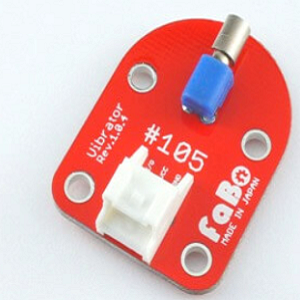
\includegraphics[width=0.5\linewidth]{images/chap05/text05-img017.png}
        \caption{振動子}
        \smallskip
      \end{minipage} &
      回路記号 & 
      \begin{minipage}[t]{\linewidth}
      \smallskip
        \centering
        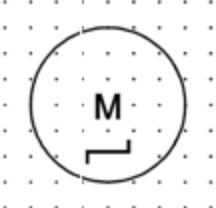
\includegraphics[width=0.5\linewidth]{images/chap05/text05-img044.png}
        \caption{振動子の回路図}
        \smallskip
      \end{minipage}\\ \hline
    \end{tabular}
  }
\end{figure}
